%!TeX encoding = UTF-8
%!TeX root = ../main.tex
\chapter{Doc of the doc}
\label{chapter:autodoc}

This chapter expains how this document structure works.
It's aimed at people who (like me) don't know much about \LaTeX.

Most of the information you'll find in the first section is a very short
substract from \url{https://en.wikibooks.org/wiki/LaTeX}.

\section{Basic composing - standard \LaTeX}

Here's what you need to know to create chapters, sections, etc.

\subsection{Basic stuff}


You have different levels in \LaTeX to generate different title structures. Here's how it works (but for additional information, check \url{https://en.wikibooks.org/wiki/LaTeX/Document_Structure}).

\begin{lstlisting}[style=Latex-color]
\chapter{This is a chapter}
A chapter starts on a blank page.
Use chapter* in your forewords to exclude them for table of contents.
\section{Big title}
Usually this is what we call level-2 title.
\subsection{Subsection}
This is a subsection content
\subsubsection{Subsubsección}
Guess what it is?
\paragraph{A very deep level}
Here's the paragraph content. See how its content starts on the same line as the title.
\end{lstlisting}
This is how it looks:
    \section*{Big title}
    Usually this is what we call level-2 title.
    \subsection*{Subsection}
    This is a subsection content
    \subsubsection*{Subsubsección}
    Guess what it is?
    \paragraph*{A very deep level}
    Here's the paragraph content. See how its content starts on the same line as the title.

Apart from that, linebreaks are ignored. To separate paragraphs, use a blank line.

For example, this is a new paragraph.


This is a new paragraph on a separated blank line.

\subsection{Footnotes}

\todo{Document this}

\subsection{Glossary}

See the \texttt{glossary.tex} file that explains all by examples.

\section{Fancy stuff (images, highlighting)}

\subsection{Images}

Put your images in the \texttt{assets} directory. Then use the following code:

\begin{lstlisting}[style=Latex-color]
\begin{figure}
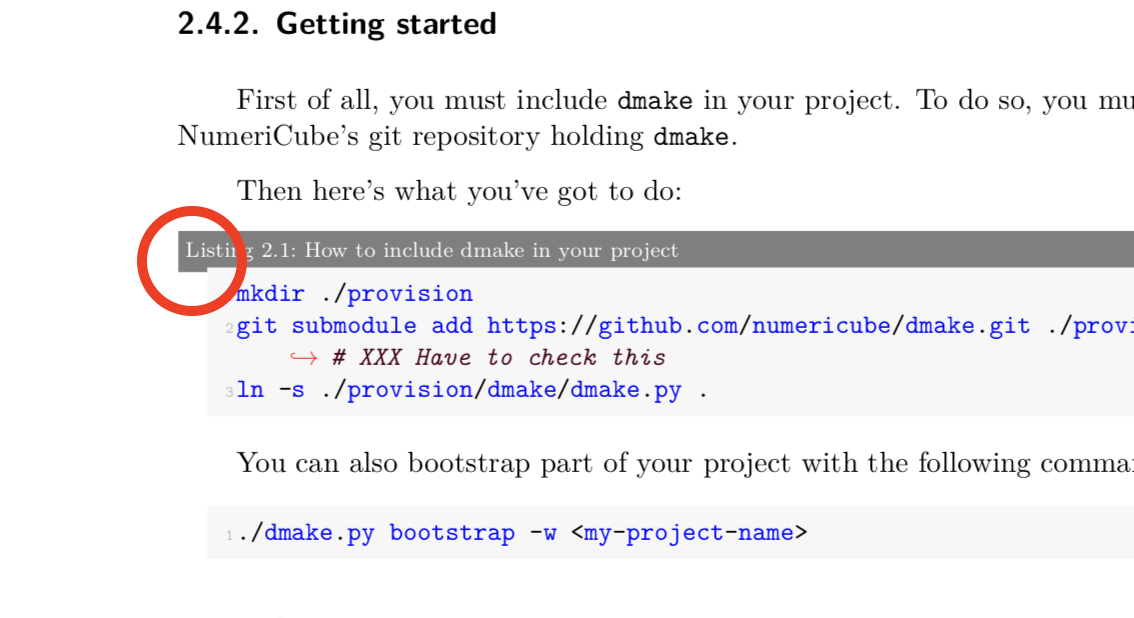
\includegraphics[width=\textwidth]{assets/alignmentpb.png}
\caption{Alignment problem}
\end{figure}
\end{lstlisting}

\subsection{Pretty boxes}

You can include pretty boxes with the \texttt{\textbackslash warningbox} directive.

\begin{lstlisting}[style=Latex-color]
\warningbox{This is a warning box.}
\end{lstlisting}

\warningbox{This is a warning box.}

For the record, here's the list of available boxes from the package:

\begin{lstlisting}[style=Latex-color]
\notebox{\lipsum[2]}
\tipbox{\lipsum[3]}
\warningbox{\lipsum[4]}
\cautionbox{\lipsum[5]}
\importantbox{\lipsum[6]}
\end{lstlisting}

\subsection{CSV files}

This is how to add a big CSV file.
\todo{Use the new format for tables (see \texttt{history.tex} file).}
For the record, this was generated with \texttt{git log \-\-date=local \-\-pretty=format:"\%h\%x09\%an\%x09\%ai\%x09\%s"}

\csvautolongtable[
    separator=tab,
    % no head,
    respect all
]{assets/commits.csv}
% {1=\hash,2=\author,3=\date,4=\comment}
% {\hash & \author & \date & \comment}


\section{Pretty schemas (using \texttt{TikZ})}

Ok let's admit it: drawing with \texttt{TikZ} in a complete abstract environment is a nightmare.

However, you can create a (free) account on \url{https://www.overleaf.com}, open the Drawing example
(\url{https://www.overleaf.com/latex/examples/hello-world-example/hthgmnnxbhhx}) and start fiddling
from there.

We provide a few examples of what we can do with styles included with the present document.

Figure \ref{figure:smpreleaseworkflow} provides an example of such a schema.

\begin{lstlisting}[style=Latex-color,caption={my-listing}]
\begin{figure}
\centering
\begin{tikzpicture}[node distance=2cm,
    every node/.style={fill=white, font=\sffamily}, align=center]
    \node (init)                [textbox0]
        {textbox0\\This is the textbox content};
    \node (write)               [textbox1, below of=init]
        {textbox1\\This is the textbox content};
    \node (testCode)            [textbox3, below of=write]
        {textbox3};
    \node (commitCode)          [textbox4, below of=testCode]
        {textbox4};
    \node (release)             [textbox1, below of=commitCode]
        {textbox5};
    \node (generate)            [textbox3, below of=release]
        {textbox3};

    \node (repeat) [right of=testCode,xshift=5cm]
           {Rinse, repeat};
    \draw[arrow]         (init) -- (write);
    \draw[arrow]         (write) -- (testCode);
    \draw[arrow]         (testCode) -- (commitCode);
    \draw[arrow]         (commitCode) -- (release);
    \draw[arrow]         (release) -- (generate);
    \draw[arrow]        (generate) -| (repeat);
    \draw[arrow]        (repeat) |- (init);
\end{tikzpicture}
\caption{Description of the overall release textbox1}
\label{figure:smpreleaseworkflow}
\end{figure}
\end{lstlisting}

% Workflow for development activites
\begin{figure}
\centering
\begin{tikzpicture}[node distance=2cm,
    every node/.style={fill=white, font=\sffamily}, align=center]
    \node (init)                [textbox0]
        {textbox0\\This is the textbox content};
    \node (write)               [textbox1, below of=init]
        {textbox1\\This is the textbox content};
    \node (testCode)            [textbox3, below of=write]
        {textbox3};
    \node (commitCode)          [textbox4, below of=testCode]
        {textbox4};
    \node (release)             [textbox1, below of=commitCode]
        {textbox5};
    \node (generate)            [textbox3, below of=release]
        {textbox3};

    \node (repeat) [right of=testCode,xshift=5cm]
           {Rinse, repeat};
    \draw[arrow]         (init) -- (write);
    \draw[arrow]         (write) -- (testCode);
    \draw[arrow]         (testCode) -- (commitCode);
    \draw[arrow]         (commitCode) -- (release);
    \draw[arrow]         (release) -- (generate);
    \draw[arrow]        (generate) -| (repeat);
    \draw[arrow]        (repeat) |- (init);
\end{tikzpicture}
\caption{Description of the overall release textbox1}
\label{figure:smpreleaseworkflow}
\end{figure}



% ISO 62304 activities
\begin{figure}
\centering
\begin{tikzpicture}[node distance=2cm,
    every node/.style={fill=white, font=\sffamily}, align=center]

    \node (section61)                [textbox1]
        {Software maintenance plan};
    \node (section62)               [textbox1, below of=section61]
        {Problem and modification analysis};
    \node (section53)            [textbox2, below of=section62]
        {Software architectural design};
    \node (section54)          [textbox1, below of=section53]
        {Software detailed design};
    \node (section55)             [textbox0, below of=section54]
        {Software unit implementation and verification};
    \node (section56)            [textbox1, below of=section55]
        {Software integration and integration testing};
    \node (section57)            [textbox3, below of=section56]
        {Software system testing};
    \node (section58)            [textbox1, below of=section57]
        {Software release};
    \draw[arrow]         (section61) -- (section62);
    \draw[arrow]         (section62) -- (section53);
    \draw[arrow]         (section53) -- (section54);
    \draw[arrow]         (section54) -- (section55);
    \draw[arrow]         (section55) -- (section56);
    \draw[arrow]         (section56) -- (section57);
    \draw[arrow]         (section57) -- (section58);

\end{tikzpicture}
\caption{Description of the overall release\\
\legendzero\ White dot that is used to show something that's white.\\
\legendone\ Same with a \texttt{textbox1} text, etc
}
\label{figure:smpreleaseworkflow}
\end{figure}


\section{Todo list}

If you ever need to mention things to do, use the following:

\begin{lstlisting}[style=Latex-color]
\todo{Thing not to forget}
\missingfigure{Figure you need to include}
\todo[inline]{An inline todo note}
\end{lstlisting}

With the default template, todos are automatically indexed at the end of your document.

\subsection{Miscellaneous stuff}

\begin{itemize}
    \item Change BW page to something like this \url{https://www.latextemplates.com/templates/books/2/book_2.pdf} (look at page 3)
    \item Add a backcover page (even if it's just white)
    \item Mention the excellent base template in acknoledgements: \url{https://github.com/jmrplens/TFG-TFM_EPS}
\end{itemize}

\subsection{Caption alignment error}

There's a slight alignment error with code captions when using \texttt{lstlisting} (see screenshot below). It has to be fixed.

\begin{figure}
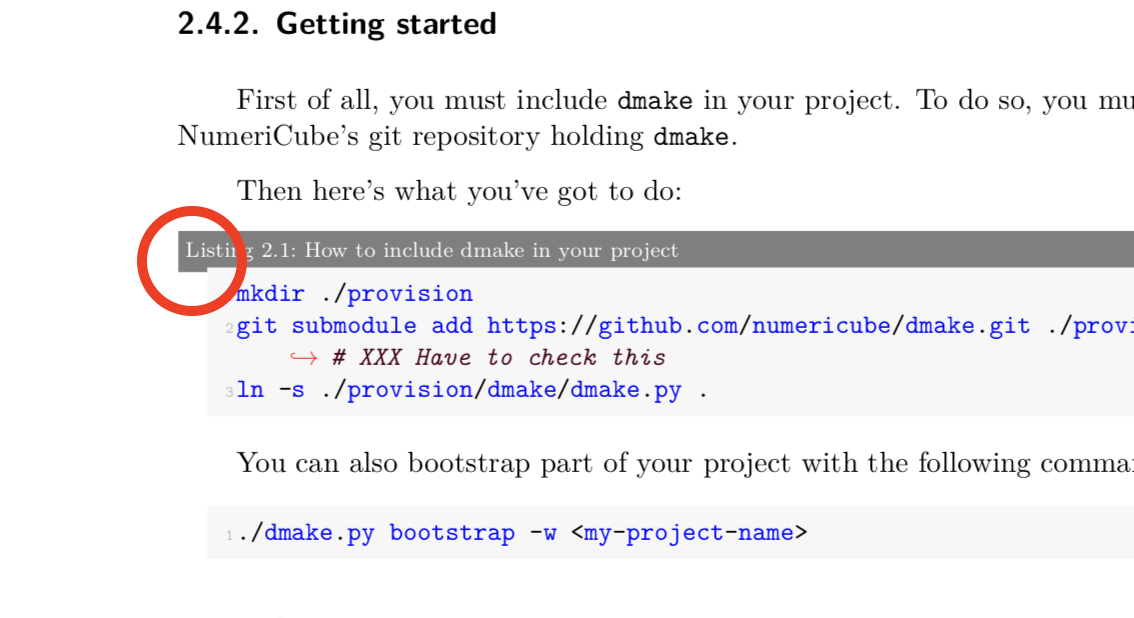
\includegraphics[width=\textwidth]{assets/alignmentpb.png}
\caption{Alignment problem}
\end{figure}


\subsection{Logos}

Logo management is far from perfect, especially on the front page (oops).

Probably need someone to make PDF-compliant EPS versions of my logo in various versions. See table \ref{table:logoformats} on page \pageref{table:logoformats} for a complete list of what we need.

\begin{table}[ht]
	\centering
	% {\scalefont{0.9}
	\begin{tabular}{@{}lccc@{}}
	\toprule
        Filename                        &   Baseline Language   &   Shape   & Base color \\ \midrule
        LogoN3-2018-EN-rect-white       &   English             & Rectangle & White/Transparent \\
        LogoN3-2018-FR-rect-white       &   French              & Rectangle & White/Transparent \\
        LogoN3-2018-EN-square-white     &   French              & Square    & White/Transparent \\
        LogoN3-2018-FR-square-white     &   French              & Square    & White/Transparent \\
        LogoN3-2018-EN-rect-black       &   English             & Rectangle & Black/Transparent \\
        LogoN3-2018-FR-rect-black       &   French              & Rectangle & Black/Transparent \\
        LogoN3-2018-EN-square-black     &   French              & Square    & Black/Transparent \\
        LogoN3-2018-FR-square-black     &   French              & Square    & Black/Transparent \\ \bottomrule
	\end{tabular}
	% }
	\caption{Different types of logos to have in the \texttt{include/logos} folder.}
	\label{table:logoformats}
\end{table}

\subsection{.gitignore}

We should document what should be in \texttt{.gitignore} (and not into git, then).

Ideas comming in mind:

\begin{itemize}
    \item \texttt{docgen} folder
    \item \texttt{build} folders
    \item \texttt{provision/history} folder (or maybe not?)
    \item \texttt{DS\_Store} Mac Finder folders
\end{itemize}

\section{Lorem ipsum (just to check text structure)}

\lipsum
